\atspt
\begin{frame}{\ft{Common Plugin Functionality}}
\section{MPF -- Common Functionality}
\doubleFrame{MPF Plugins have similar functionality and 
features in different host applications, which makes 
it convenient to use as readers switch among multiple applications.}

\vspace*{2pt}\hspace*{8pt}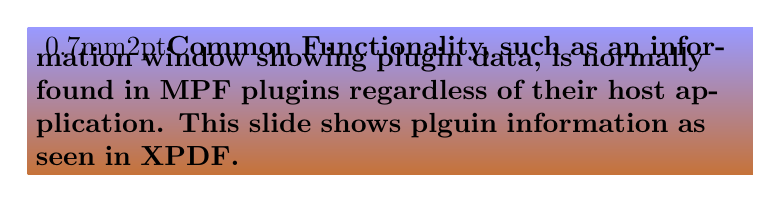
\begin{tikzpicture}
\nodeincludegraphicsTRRS{1.125}{0cm}{1cm}{0cm}{0cm}{after/mpf-3.png}

 \node [anchor=west,bottom color=brown!90!red,top color=blue!40, inner sep=3, text width=9cm]
  (longnote) at (21.5,10) {\vspace{-8pt} %  %{\color{rb!85!red}{
  {\cframedboxx{0.7mm}{2pt}{\annfont\textbf{Common 
Functionality, such as an information window showing plugin 
data, is normally found in MPF plugins regardless 
of their host application.  This slide shows 
plguin information as seen in XPDF.}}}};

\ann{darkRed}{1}{.8mm}{grammarArrowColor}{0.5}{7.1,13.9}{1.4}{.6}{0.7}

\curicon{22}{4.8}

\end{tikzpicture}


\end{frame}

